\chapter{Detecting exoplanets with the transit method}

%TODO have TAs take data a couple weeks in advance, so they get experience with the whole process.
%TODO instead of each group doing a different system, have the whole lab section do one system and split the observations across different groups, to reduce tedium and simulate being part of a larger research group.

Over the next two weeks, you will learn how to use the transit method to detect exoplanets. You will use    one    of    the    MicroObservatory    telescopes,    built    and    maintained    by    the    Harvard‐Smithsonian    Center    for    Astrophysics    and    located    at    the    Whipple    Observatory    in    Amado,    Arizona    to    take    a    series    of    images    of    a    ``target''    star in order to calculate a light curve for that star, which could be used to learn about the planet(s) orbiting them.    These    images    will    form    the    basis    of    your    subsequent    investigation in the Image Lab on the LSE website.

\section{Scheduling observations}

First, schedule the remote observations. The observations are made at night in Arizona, and they can be scheduled during the day before those observations.

\begin{steps}
	\item Find the transit calendar in the Lab 3 Files folder in the Files section on Canvas. Pick an exoplanet transit that will be observable sometime during the next two weeks. Note that all times listed here are local to Arizona.
	
	\item Log into the exoplanet lab website at \url{https://www.cfa.harvard.edu/smgphp/otherworlds/ExoLab/index.html} using the username and password your TA has given you. If you haven't received this yet, skip this section until you receive it.
	
	\item Click "Go to the lab", and then select the Telescope tab. Go through the sections on the right side of the page to learn
	about the remote observatory we are using and how to schedule observations.
	
	\item On the day before the transit is observable, go to this website and schedule your observations. Each transit will require observing for $\approx 1\:$hour before and $\approx 1\:$hour after the
	transit for a total observation time of 4--5 hours. This corresponds to 80--100 exposures. You can split this effort among your group mates, each scheduling under their own user name.
\end{steps}

\section{Tutorials and analysis}

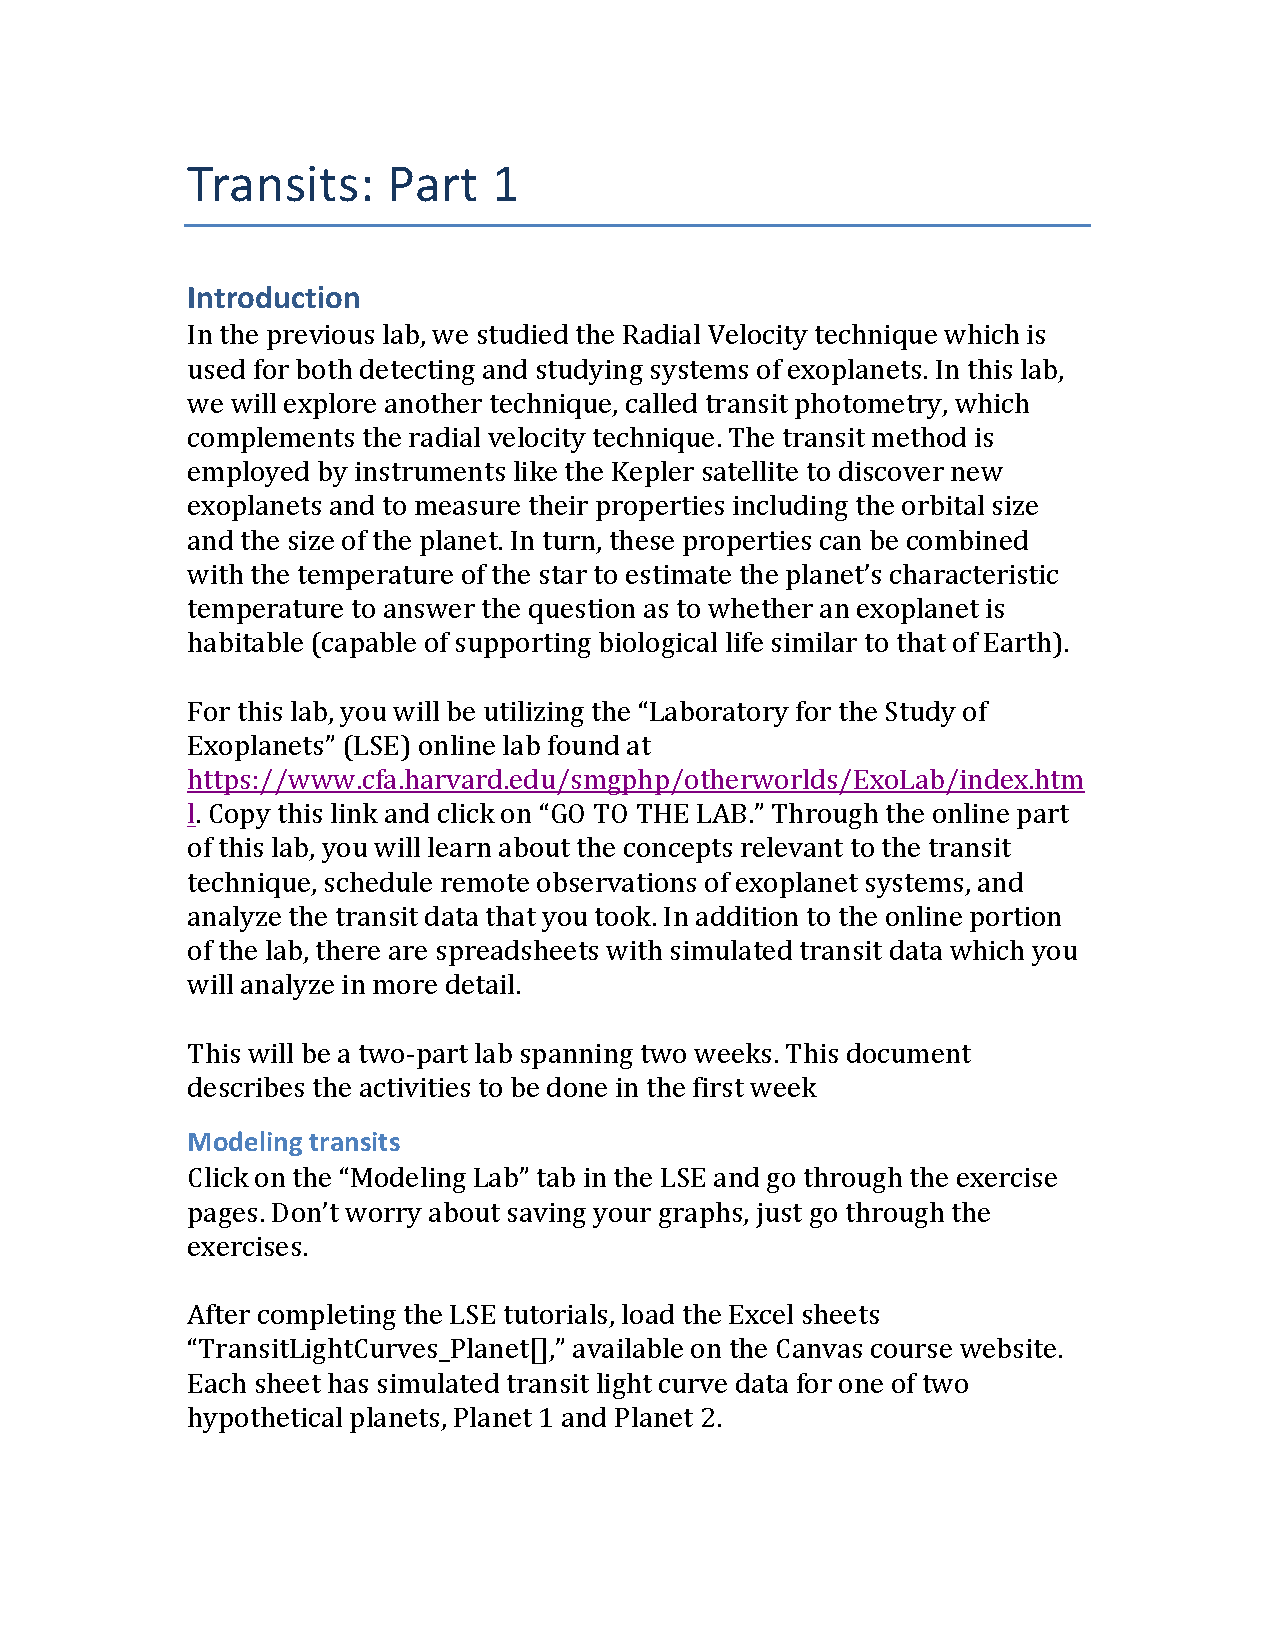
\includepdf[pages=1-4]{transits/transits-part-1}

\section{Analyzing your own data}

You will use the LSE website to analyze an example image, then can analyze your own images for the report.

\begin{steps}
	\item Click on the “Image Lab” and go through the 9 page tutorial. Practice
your analysis on the “Demo\_Images” for TRES-3. Make sure you subtract
and appropriate Dark Image (note that the image filenames include the
date and time of the exposure).

	\item Once it’s been taken, analyze the data from your scheduled
observations. Be sure to press the “Calculate \& Record” button to save
your results.

	\item Combine your data with the rest of your group by looking at the “class graph.” \textbf{Save this light curve and turn it in with your write up.}

\end{steps}

\section{Report checklist and grading}

Each item below is worth 10 points.

\begin{enumerate}
	\item Data table from Part 1.
	
	\item Plots of your light curves for Planet 1, Planet 2, and the planet you observed with LSE. 
	
	\item Discuss how different features of the light curve connected to physical
	properties of the orbital system.
	
	\item Your calculated temperature for Planet 1 and Planet 2, and your interpretation of the
	temperatures for the simulated planets.
	
	\item List which scheduled observations your group performed. Were you able to see a light curve from your scheduled observations? Why or why not?
	
	\item A 100--200 word reflection on group dynamics and feedback on the lab manual. Address the following topics: who did what in the lab, how did you work together, what successes and challenges in group functioning did you have, and what would you keep and change about the lab write-up?
\end{enumerate}